\section{Stochastic inference of surface-induced effects using Brownian motion}

\subsection{Confined Brownian motion theory}

By observing the trajectory along the $z$ axis of a particle of $1.5 ~ \mathrm{\mu m} $ as shown on the fig.\ref{Fig:exp_z_traj}, one can see that the particle height does not get heigher than $ \simeq 4 ~ \mathrm{\mu m}$. Indeed due to gravity, the particle is confined near the surface. Brownian motion in confinement and at interfaces is a canonical situation, encountered from fundamental biophysics  to  nanoscale  engineering. This confinement induces near-wall effects, such as hindered mobility and electrostatic interactions. 

In the first part of this chapter, I will detail the theory background of the confined Brownian motion and how to numerically simulate it. In a second part, I will present how to analyse experimental data. In particular, I will detail a multi-fitting procedure that allows a thermal-noise-limited inference of diffsion coefficients spatially resolved at the nanoscale, equilibrium potentials, and forces at the femtomewton resolution.

\begin{figure}[ht]
	\centering
	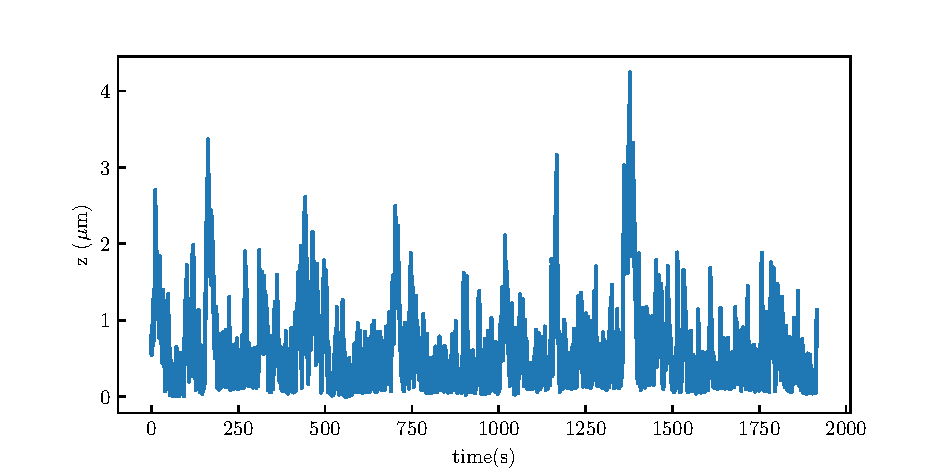
\includegraphics{02_body/chapter3/images/traj_z/traj_z.pdf}
	\caption{Experimental trajectory of a particule of polystyrene of radius $a = 1.5 ~ \mathrm{\mu m}$ near a wall ($z = 0$) along the $z$ axis --- perpendicular to the wall.}
	\label{Fig:exp_z_traj}
\end{figure}

\subsubsection{Gravitational interactions}


In our experiment, we observe confined Brownian motion since the colloids are subject to gravity. Indeed, the density of the observed colloid $\rho_\mathrm{p}$ is different of the medium $\rho_\mathrm{m}$ --- in our experiment water, $\rho_\mathrm{m} = 1000 ~ \mathrm{kg.m^{-3}}$. Thus, the particle lies into a gravitational potential given by:

\begin{equation}
	U_\mathrm{g} (z) = \Delta m g z = \frac{4}{3}\pi a ^3 g \Delta \rho z ~,
	\label{eq:ug_full}
\end{equation}

where $\Delta m$ is the mass difference of the particle and a fluid sphere of the same size, $\Delta \rho$ the corresponding density difference such as $\Delta \rho = \rho_\mathrm{m} - \rho_\mathrm{p} $ and $g$ the gravitational acceleration. By invoking the definition of a distance that we call the Boltzmann length,

\begin{equation}
	\ell _\mathrm{B} = \frac{k_\mathrm{B}T}{4/3 \pi a ^3 \Delta \rho g } ~,
\end{equation}

one can rewrite the gravitational potential Eq.\ref{eq:ug_full} as:

\begin{equation}
	U_\mathrm{g} = \frac{k_\mathrm{B}T}{\ell _\mathrm{B}} ~.
	\label{eq:ug}
\end{equation}

The Boltzmann length $\ell_\mathrm{B}$ is the typycal gravitational decay length and represents the balance between the gravital potential and thermal energy. This distance was first measured by Perrin \cite{perrin_les_2014}, by enumerating the number of particles as a function of height to reconstruct the concentraction of the colloidal suspension that exponentially decays as $e^{- z / \ell _\mathrm{B}}$. As an exemple, in water, for a particle polystyrene, $\rho _\mathrm{p} = 1050 ~ \mathrm{kg.m^{-3}}$ and of radius $a  = 1.5 ~ \mathrm{\mu m}$ we have $\ell _\mathrm{B} = 0.58 ~ \mathrm{\mu m}$.

For particle with $\ell _\mathrm{B} >> a $, one can consider that the particle does not feel the gravity. This is particulary the case when the density of the colloids and fluid matches, in this particular case $\ell _\mathrm{B} = 0$. Thus density matching can we a way to do grativation free experiments. In the case of our experiment, we want to measure confinement induced effects, therefore, we need this gravitational interaction to have the particles near the surface. Indeed, as a particle gets larger, or, denser $\ell _\mathrm{B}$ decreases and the particle will be, in average, closer to the surface. 


\subsubsection{Sphere-wall interactions}

As we have seen, external forces acts on the particle such as the gravity, however it is not the only one. As the Brownian particle is close to a wall we can expect some interactions between the surfaces. In our case, we suppose that the Brownian particles do not interact between each other, which is the case for the dilute solution used. Indeed, the particles studied are at a minimum $50 ~ \mathrm{\mu m}$ apart which correspond to 10 times their size for the larger beads. 

To describes the interaction between, the Brownian particle and the wall, we use the DLVO\footnote{The DLVO theory is named after Derjaguin, Landau, Verwey, and Overbeek \cite{israelachvili_intermolecular_2015}.} theory. This theory was first developed to describe the interactions between colloids to explain the stability of colloidal suspension. It describes the interactions using two forces components; the Van Der Waals force which arise form the interactions between surface's molecules and electrostatic interactions due the a double-layer formed with the ions present in the solution. 

\paragraph{Double-Layer interactions}\mbox{}\\
\vspace{0.10cm}


When a surface is immersed in water are usually charged \cite{israelachvili_intermolecular_2015} due to a high dielectric constant $\epsilon \simeq 80$ that permit the build up of charges for low energetic price. Commonly, surface charging is done through ionization of dissociation of surface groups\footnote{For example, the dissociation of protons from surface carboxylic groups \cite{israelachvili_intermolecular_2015} ($-$COOH $\rightarrow$ -COO$^-$ + H$^+$) which charge negatively the surface.}, from the binding of ions from the solution --- for example, adsorption of $-$OH$^-$ onto the water-air interface that charge it negatively. In the bulk, a fluid should be electrically neutral, thus the fluid contains as many ions of opposite charge. However, when a surface is charged negatively, negative ions are repelled from the surface, while positive ions are attracted towards the surface.  Therefore, a double-layer charge distribution is formed near the surface, as shown Fig.\ref{fig.taumax}-a). Experimentally, we use glass slides and polystyrene beads, that are both negatively charged in water, thus leading to repulsive double-layer. This repulsive force prevent the colloids to stick together or to the surface of the substrate. 






\begin{figure}[h]
	\centering
	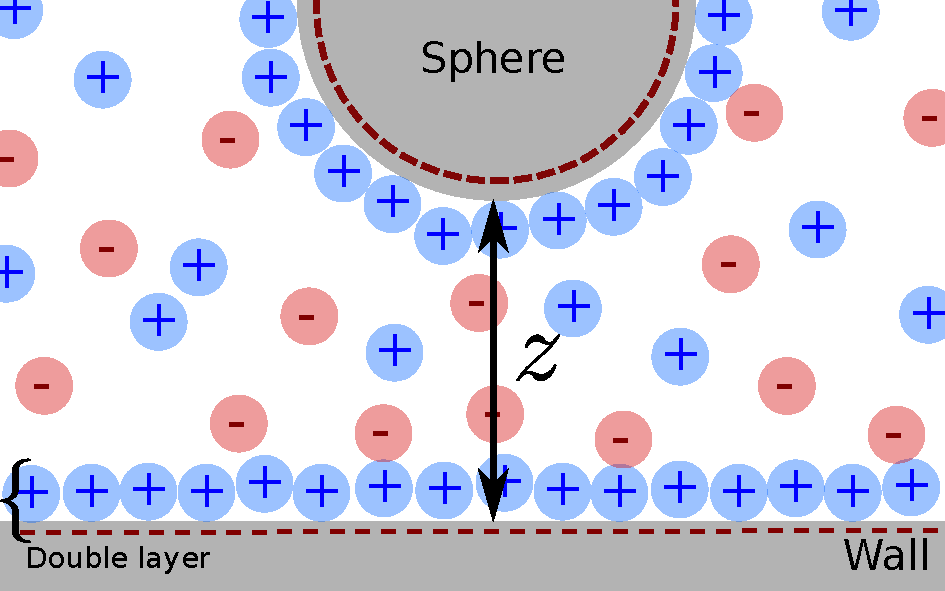
\includegraphics{02_body/chapter3/images/double_layer.pdf}
	\caption{A Brownian colloid diffusing near a wall. Both wall and colloid's surface charge negatively, in consequence, a layer of positively charge ions are towards the surfaces, forming a double-layer charge distribution.}
	\label{Fig:double_layer}
\end{figure}




If the solution contains an electrolyte (ions of positive and negative charges), for example a salty solution, containing Na$^+$ and Cl$^-$ ions. In the DLVO theory, the electrostatic field $\Psi(\vec{r})$ generated by the double layer satisfies the mean field Poisson's equation \cite{israelachvili_intermolecular_2015}:

\begin{equation}
	\nabla ^2 \Psi(\vec{r}) = -\frac{1}{\epsilon_r \epsilon_0}  \rho_e(\vec{r})~,
	\label{Eq:poisson}
\end{equation}

where $\epsilon_0$ the vacuum permittivity, $\epsilon_r$ the relative permitivity of the fluid, $\rho_e(\vec{r})$ the local charge density. The latter can be written as:

\begin{equation}
	\rho_e(\vec{r}) = e \sum _i z_i c_i (\vec{r}) ~,
	\label{Eq.3}
\end{equation}

where $e$ is the elementary charge, $i$ denotes an ionic species of valence $z_i$ and local ionic concentration $c_i(\vec{r})$ (number density). If the solution is at the thermodynamic equilibrium, the Boltzmann equation is used to calculate the local ion density such that:

\begin{equation}
	c_i(\vec{r}) = c_i ^0 \textnormal{exp}\left(\frac{z_i e \Psi(\vec{r})}{k_\mathrm{B} T }\right) ~,
	\label{Eq.4}
\end{equation}


where $c_i ^0$ is the bulk concentration (number density) of the ionic species $i$. By combining Eqs.\ref{Eq:poisson}, \ref{Eq.3} and \ref{Eq.4}, one can obtain the Poisson-Boltzmann equation:

\begin{equation}
	\nabla ^2 \Psi (\vec{r}) = \sum_i \frac{z_i e c_i^0}{\epsilon_0 \epsilon_r} \exp \left( - \frac{z_i e \Psi (\vec{r})}{k_\mathrm{B}T} \right) ~.
	\label{Eq:Poisson-boltzmann}
\end{equation}

Since the Poisson-Boltzmann is non-linear, it is most likely to be solve numerically. However, for simple geometry such as uniformly charged plane or sphere it can be solve analiticaly. Let consider, to simplify, that we have a monovalent electrolyte, meaning that the electrolyte is composed of two ions of valence equal to one --- Na$^+$ Cl$^-$ for example --- and $c_i ^0$ is equal to the electrolyte solution concentration $c_s^0$. In that case Eq.\ref{Eq:Poisson-boltzmann} simplifies to:

\begin{equation}
	\begin{aligned}
	\nabla ^2 \Psi (\vec{r}) &= \frac{e c_s ^0}{\epsilon_0 \epsilon_r} \left[ \exp \left( \frac{-e\Psi(\vec{r})}{k_\mathrm{B}T} \right) -  \exp \left( \frac{+e\Psi(\vec{r})}{k_\mathrm{B}T} \right) \right] \\
	& = 2 \frac{e c_s ^0}{\epsilon_0 \epsilon_r} \mathrm{sinh}  \left( \frac{e\Psi(\vec{r})}{k_\mathrm{B}T} \right) ~.
	\end{aligned}
\end{equation}

In the case, where the $\Psi$ is small enough everywhere to have the electrostatic potential energy $e\Psi << k_\mathrm{B} T$, which generally the case when using salty solution. In that case, it is possible, using the a Taylor approximation at the second order to write:

\begin{equation}
	\exp \left( - \frac{z_i e \Psi(\vec{r})}{k_\mathrm{B}T} \right) \simeq 1 + \frac{z_i e \Psi (\vec{r})}{k_\mathrm{B}T} ~.
\end{equation}

Thus, the Poisson-Boltzmann equation (Eq.\ref{Eq:Poisson-boltzmann}) becomes:

\begin{equation}
	\nabla ^2 \Psi (\vec{r}) = \sum_i \frac{z_i e c_i^0}{\epsilon_0 \epsilon_r}  \left( 1 + \frac{z_i e \Psi (\vec{r})}{k_\mathrm{B}T} \right) ~.
\end{equation}

Since the fluid in the bulk, is electrically neutral, the first term vanishes as $\sum_i z_i c_i^0 = 0$. One thus have a linearized version of Eq.\ref{Eq:Poisson-boltzmann}, which is known as the Debye-Hünkel equation:

\begin{equation}
	\nabla^2 \Psi (\vec{r}) = \left[  \sum_i \frac{z_i ^2 e^2 c_i^0}{\epsilon_0 \epsilon_r  k_\mathrm{B} T}    \right] \Psi (\vec{r}) ~.
\end{equation}

From this approximation, one can identify that the term between brackets is the inverse of a distance squared. We can thus define a distance $\ell _\mathrm{D}$, the Debye length such as:

\begin{equation}
	\ell _\mathrm{D} =  \sqrt{ \sum_i\frac {\epsilon_0 \epsilon_r k_\mathrm{B} T} {z_i ^2 e^2 c_i^0}} ~.
\end{equation}

The Debye length is the characteristic length of the double-layer, and, the electrostatic interactions. For a monovalent electrolyte,  at 25 \textdegree C (298 K), the Debye length of aqueous solution is:

\begin{equation}
	\begin{aligned}
		\ell _\mathrm{D} &= \sqrt{\frac{\epsilon_0 \epsilon_r k_\mathrm{B}T}{2c_s^0 e^2}}
		= \sqrt{\frac{8.854 \times 10^{-12} \times 78.4 \times 1.381 \times 10^{-23}  \times 298}{2 \times (1.602 \times 10^{-19})^2 \times 6.022 \times 10^{26} M}} \\
		& = 0.304 \times 10^{-9} / \sqrt{M} ~ \mathrm{m} ~,
	\end{aligned}
\end{equation}


with M the molar concentration ($1 ~ \mathrm{M} = 1 ~ \mathrm{mol.L^{-1}} $ corresponding to a number density of $c_s^0 = 6.022 \times 10 ^{26} ~ \mathrm{ m^{-3}}$). Thus, for a salty concentration we have
 $\ell_\mathrm{D} = 0.304/ \sqrt{[\mathrm{NaCl}]} ~ \mathrm{nm}$. For exemple, for NaCl solution, one can have $\ell_\mathrm{D} = 100 ~ \mathrm{nm}$ for a concentration  $[\mathrm{NaCl}] = 9.2 ~ \mathrm{\mu M}$ and   $\ell_\mathrm{D} = 10 ~  \mathrm{nm}$ for a concentration  $[\mathrm{NaCl}] = 9.2 ~ \mathrm{mM}$.



Finally, the Debye-Hünkel approximation finally writes:

\begin{equation}
	\nabla^2 \Psi (\vec{r}) = \kappa^2  \Psi (\vec{r}) ~,
	\label{Eq:Debye_hu}
\end{equation}

with $\kappa = 1/\ell _\mathrm{D}$. Using the latter approximation one can compute the electrostatic potential around a sphere. Let us consider a perfect sphere of radius $a$ and charge $Qe$ of charge density $\sigma = Qe/4\pi a^2$. With $Q$ beeing the number of charge on the surface. Since the system has a spherical symmetry, one has $\Psi (\vec{r}) = \Psi(r)$ with $r = |\vec{r}|$. Using the Laplacian operator $\nabla ^2$ in the spherical coordinates, Eq.\ref{Eq:Debye_hu} writes:

\begin{equation}
	\frac{1}{r^2}\left[\frac{\partial}{\partial r} \left(r^2 \frac{\partial \Psi(r)}{\partial r}\right)\right] = \kappa^2  \Psi (r) ~,
\end{equation}

which has a general solution:

\begin{equation}
	\Psi(r) = C_1 \frac{\exp(\kappa r)}{r} + C_2 \frac{-\exp(\kappa r)}{r}
\end{equation}

For one sphere, the electrostatic field vanishes at infinity such as $C_1 = 0$, such it has the form of a Yukawa potential:

\begin{equation}
	\Psi (r) = C_2 \frac{-\exp(\kappa r)}{r} ~.
	\label{eq:yuka}
\end{equation}

Additionally, at the surface of a charged sphere, the eletrostatic potential satifies:

\begin{equation}
\left. \frac{\partial{\Psi (r)}}{\partial r} \right|_{r=a} = \frac{Qe}{4 \pi \epsilon_0 \epsilon_r a^2}  = \frac{\sigma}{\epsilon_0 \epsilon_r} ~.
\end{equation}

By applying the latter boundary condition to Eq.\ref{eq:yuka} we find:

\begin{equation}
	\Psi (r) = \frac{\sigma a^2}{\epsilon_0 \epsilon_r} \frac{\exp (\kappa a)}{1 + \kappa a} \frac{\exp (-\kappa r)}{r}
\end{equation}

This solution can be used to determine the  electrostatic field between two spheres. Indeed, if we suppose that the presence of a second sphere, do not interfere with the distribution of ions in the double layer of the other. We can thus use the superposition approximation to write the potential $\Psi _2 (z)$ between two spheres surfaces. Where $z$ is the distance between the 2 colloids. For two spheres of charge $\sigma_1$ and $\sigma_2$ and radius $a_1$ and $a_2$, $\Psi_2 (z)$ writes \cite{bell_approximate_1970}:

\begin{equation}
	\Psi(z) = \frac{4\pi}{\epsilon_0 \epsilon_r} 
	\left(
	\frac{\sigma_1 a_1 ^2}{1 + \kappa a_1}
	\right)
	\left(
	\frac{\sigma_2 a_2 ^2}{1 + \kappa a_2}
	\right)
	\frac{\exp(-\kappa z)}{a_1 + a_2 + z} ~.
\end{equation} 

From the latter equation, it is possible to write the electrostatic field between a wall and a spherical colloid, by setting one of the radius to infinity. Doing so and mulitplying by $e$, one can have the eltrostatic potential $E_\mathrm{elec}(z)$ between a Brownian particle and the wall:

\begin{equation}
	E_{elec} (z) = B \mathrm{e}^{-\frac{z}{\ell_\mathrm{D}}}~.
	\label{Eq:Uelec}
\end{equation}

Where B is the constant that represent the surface charges, for sphere of radius $a$ and charge $\sigma_1$ and a wall of charge $\sigma_2$, one has:

\begin{equation}
	B = \frac{4 \pi}{\epsilon_0 \epsilon_r} \left( \frac{\sigma_1 a^2 }{1 + \kappa a}  \right) \frac{\sigma_2}{\kappa} ~.
\end{equation}

 Additionally, $B$ is often written as a function of the surfaces potential as [CITE PRIEVES]:

\begin{equation}
	B = 16 \epsilon_r \epsilon_0 \left(\frac{k_\mathrm{B}T}{e}\right) \tanh \left(\frac{e\phi_1}{4k_\mathrm{B}T}\right) \tanh \left(\frac{e\phi_2}{4k_\mathrm{B}T}\right) ~,
\end{equation}
 where $\phi_1$ and $\phi_2$ are the Stern potentials of the sphere and the wall surfaces. Typical values for $B$ ranges from 1 $k_\mathrm{B}T$ to $50 ~ k_\mathrm{B}T$. In our study we will keep $B$ to describe the electrostatic energy potential as it complicated to decouple the $\sigma_1$ and $\sigma_2$ when the colloid and wall's surface materials are different \cite{behrens_charge_2001}. However, this is not impossible and is the idea of future work.

\paragraph{Van der Waals interactions}\mbox{}\\
\vspace{0.10cm}

\begin{figure}[h]
	\centering
	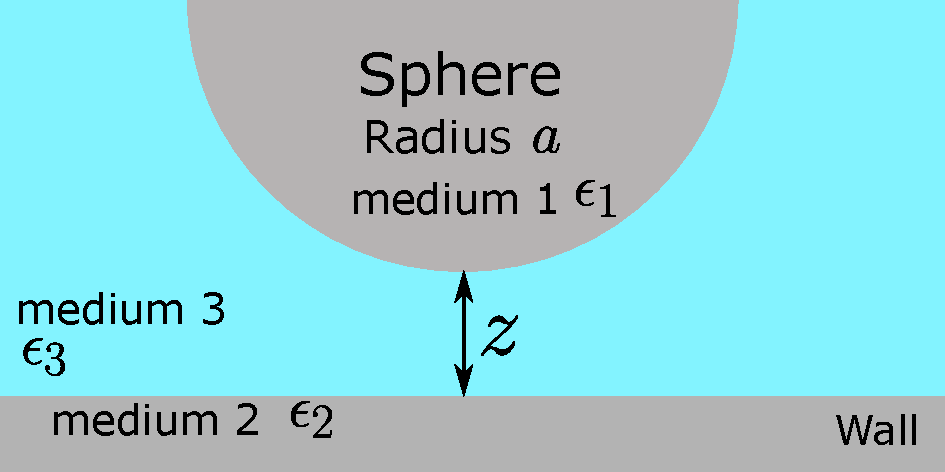
\includegraphics{02_body/chapter3/images/vdw_scheme.pdf}
	\caption{A colloid of radius $a$ separated from a wall from a distance $z$. The colloid material has a static dielectric constant $\epsilon_1$, the wall $\epsilon_2$ and the solution $\epsilon_3$. }
	\label{Fig:vdw}
\end{figure}

In the DLVO theory, the Van der Waals forces describes the interaction between colloids at very short range. This forces are mainly attractive and in our case having Van der Waals interactions would lead to the particles stick to the wall. The Van der Waals potential energy $E_{VdW}$ for a spherical colloid of radius $a$, at a height $z$  at a few nanometers ($< 5$ nm) to the surface \cite{israelachvili_intermolecular_2015}:

\begin{equation}
	E_{VdW} = -\frac{A a}{6z} 
\end{equation}

where $A$ is the retarded Hamaker constant. For our system, where the particle, medium and wall are different medium as schematize in Fig.\ref{Fig:vdw}. In that case the Hamaker constant writes \cite{israelachvili_intermolecular_2015}:

\begin{equation}
	A = \frac{3}{4} k_\mathrm{B}T \left(
	\frac{\epsilon_1 - \epsilon_3}{\epsilon_1 + \epsilon_3}
	\right)
	\left(
	\frac{\epsilon_2 - \epsilon_3}{\epsilon_2 + \epsilon_3}
	\right)
	+
	\frac{3h}{4\pi}
	\int_{\nu_1}^{\infty}
	\left(
	\frac{\epsilon_1 (i\nu) - \epsilon_3 (i\nu)}{\epsilon_1 (i\nu) + \epsilon_3 (i\nu)}
	\right)
	\left(
	\frac{\epsilon_2 (i\nu) - \epsilon_3 (i\nu)}{\epsilon_2 (i\nu) + \epsilon_3 (i\nu)}
	\right)
	\textnormal{d}\nu ~,
\end{equation}

where $\epsilon_1$, $\epsilon_2$ and $\epsilon_3$ are the static dieletric constants of the three media, $\epsilon (i\nu)$ are the imaginary dieletric constant at a frequency $\nu$ and $\nu_n = (2 \pi k_\mathrm{B}Tn/h = 4 \times 10^{13} n s^{-1}$ at $300$ K; and; h is the Plank's constant. The first term fives the zero-frequency energy of the van der Waals interaction and the second term the dispersion energy.
However, since the static dielectric of water is large compared to the other terms \cite{israelachvili_intermolecular_2015}, one can approximate the Hamaker constant of our system to only the zero-frequency term:

\begin{equation}
	A = \frac{3}{4} 1.381 \times 10^{-23} \times 298 
	\left(
	\frac{2.5 - 80}{2.5 + 80}
	\right)
	\left(
	\frac{5 - 80}{5 + 80}
	\right)
	\simeq
	2.48 \times 10^{-21} \mathrm{J}	= 0.62 ~ k_\mathrm{B}T ~.
\end{equation}

Since $A$ is positive we correctly have an attractive Van der Waals force, this case will always be the case due to the high dielectric constant of water. More over, the zero-frequency Van der Waals force is mainly due to electrostatic interaction and is thus screened by electrolytes, we thus need to add a factor $\approx e^{-z/\ell_D}$ to the Van der Waals forces. Also, it has been proposed \cite{gregory_approximate_1981} that to compute the force at higher distances, one should add a second factor, to account for the retarded Van der Waals force of $ \simeq (1  + 11z/100 \mathrm{nm})^{-1}$. 


All the effects added together we can see that the Van der Waals forces will play a role only a few nanometer ($< 10$ nm) as it is commonly observed [M,P]. In our experiments, the Debye length $\ell _\mathrm{D}$ ($>20$ nm) is large enough for the particle to avoid this region, in the following of this work the Van der Waals interactions will be neglected. To study the Van der Waals interactions with Brownian motion, it is possible, if one add enough salt to have $\ell_\mathrm{D} \simeq 1$ nm. However, with such a short Debye length, all the colloids would stick to the surface and between each other. However, we have experimentally observed some dynamics on the sucked particles, further work on this movement could lead to interesting determination of the near-wall potential. 

\newpage

\paragraph{Total potential and equilibrium distribution}\mbox{}\\
\vspace{0.10cm}

If we combine the gravitational and electrostatic interactions the particules lies into a total energy potential $U(z)$:

\begin{equation}
	U(z) = U_\mathrm{g} + U_\mathrm{elec}
	\label{eq:uz}
\end{equation}

By combining Eqs.\ref{eq:ug}, \ref{Eq:Uelec} and \ref{eq:uz}, and also adding the condition that the particle can't go inside the wall $U(z)$ finally writes:

\begin{equation}
	\frac{U(z)}{k_\mathrm{B}T} =  \left\{
	\begin{array}{l}
		\displaystyle B\,\textrm{e}^{-\frac{z}{\ell_\mathrm{D}}} + \frac{z}{\ell_\mathrm{B}}\ ,\quad \text{ for } z>0 \\
		+\infty\ ,\quad  \text{ for } z\leq 0
	\end{array}
	\right. \ ,
	\label{Eq:PDF}
\end{equation}

From this total potential energy, one can then construct the Gibbs-Boltzmann distribution to write the equilibrium \gls{PDF} of position $P_{\mathrm{eq}}(z)$:

\begin{equation}
	P_\mathrm{eq} (z)  = A \exp \left( -\frac{U(z)}{k_\mathrm{B}T} \right) ~,
	\label{Eq.Peq}
\end{equation} 

where A is a normalization constant such that $\int_{0}^{\infty}P_\mathrm{eq}(z)\textnormal{d}z = 1$. Given an array of heights $z_i$ one can use compute $P_\mathrm{eq}$ using the following Python snippet, where the $A$ is computed using the \mintinline{python}{np.trapz} function. An example of a theoretical energy potential and \gls{PDF} of position can be seen Fig.\ref{Fig:potential} for $\ell_\mathrm{B} = 500 ~ \mathrm{nm} $,  $B = 4 ~k_\mathrm{B}T$ and $\ell_\mathrm{D} = 50 ~ \mathrm{nm}$.

\begin{minted}
	[
	frame=lines,
	framesep=2mm,
	baselinestretch=1.2,
	fontsize=\footnotesize,
	linenos
	]
	{python}
import numpy as np

def _Peq(z):
  if z <= 0:
    return 0
  else:
    return np.exp(-(B * np.exp(-z / ld) + z / lb))


def Peq(z):
  P = np.array([_Peq(zi) for zi in z])
  return P / np.trapz(P,z)
\end{minted}



\begin{figure}[h]
	\centering
	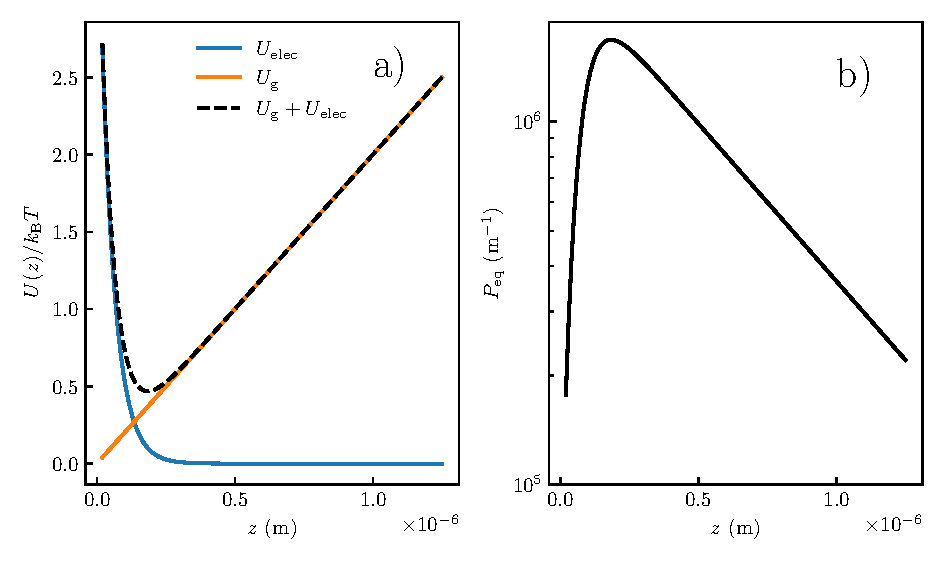
\includegraphics{02_body/chapter3/images/potential/potential_exemple.pdf}
	\caption{ a) Potential energy of a colloid of Boltzmann length $\ell_\mathrm{B} = 500 ~ \mathrm{nm} $. The electrostatic potential $U_\mathrm{elec}$ is here characterized by a surface charge constant $B = 4 ~k_\mathrm{B}T$ and a Debye length $\ell_\mathrm{D} = 50 ~ \mathrm{nm}$. b) Corresponding Gibbs-Boltzmann equilibrium distribution of position. }
	\label{Fig:potential}
\end{figure}

\subsubsection{Local diffusion coefficient}

\begin{figure}
	\centering
	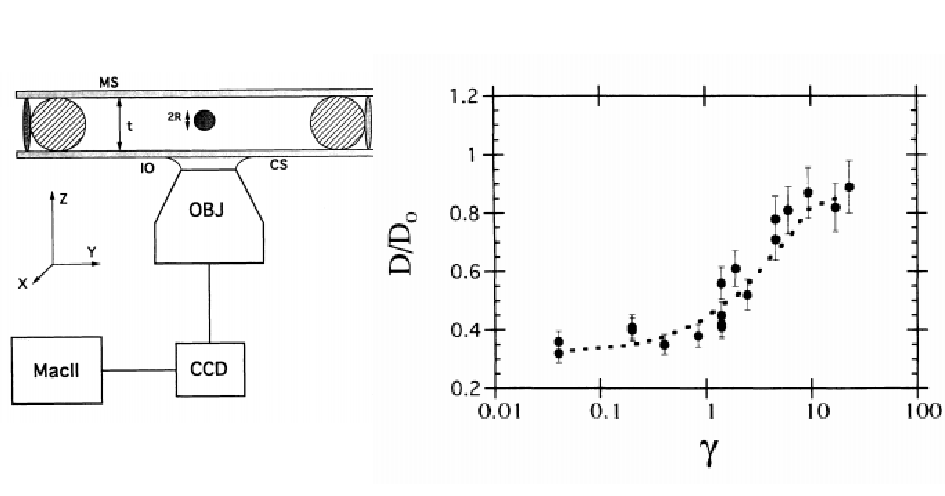
\includegraphics{02_body/chapter1/image/libchaber.pdf}
	\caption{Figure extracted from \cite{faucheux_confined_1994}, on the left is the experimental setup used. It is an inverted microscope used in order to track particle of size $2R$ inside a cell of thickness $t$. On the right is their final result, where they measure the diffusion parallel coefficient $D_\bot$ given by Eq.\ref{Eq:etax}, here normalized by $D_0$ the bulk diffusion coefficient as a function of  $\gamma$ a confinement constant $\gamma = (\langle z \rangle -a)/a$. }
	\label{fig:libchaber}
\end{figure}


As we have seen in the Chapter 2, for a freely diffusing colloid in bulk the diffusion coefficient is given by Eq.\ref{Eq:D_einstein} and is a constant. However, when a particle is confined, the diffusion is hindered, this means that the diffusion coefficient vary with the height of the particle and becomes anisotropic. One of the first measurement that has been done by Faucheux and Libchaber \cite{faucheux_confined_1994}. As we can see on the Fig.\ref{fig:libchaber}, using a microscope, they tracked Brownian colloids in two dimensions, and, measured the average coefficient diffusion for different confinement constant $\gamma = (\langle z\rangle_t - a) / a$. Finally, on the Fig.\ref{fig:libchaber}, one can observe that the diffusion coefficient parallel to the surface decreases as the particle get closer to the wall, and, seems to saturate around $0.3D_0$ for high confinement. 
\newpage

To understand the reason of this hindered diffusion coefficient, let us start by writing the diffusion coefficient $D$ using the fluctuation dissipation theorem:

\begin{equation}
	D = \mu k_\mathrm{B}T ~,
	\label{Eq.fluc}
\end{equation}

with:

\begin{equation}
	\mu = \frac{v_\mathrm{sphere}}{F_\mathrm{drag}} ~,
	\label{Eq.mu}
\end{equation}

where $v_\mathrm{sphere}$ is the terminal velocity to an applied force $F_\mathrm{drag}$. For a spherical colloid of radius $R$ moving at a velocity $v_\mathrm{sphere}$ the drag force in bulk $F_{\mathrm{drag}} ^\mathrm{B}$ is given by the Stockes' law:

\begin{equation}
	F_\mathrm{drag} ^\mathrm{B} = c \pi \eta a v_\mathrm{sphere} ~,
	\label{Eq.drag}
\end{equation}

where $c$ is a constant that depends on the boundary conditions imposed at the surface of the colloid, typically $c = 6$ for no-slip  and $c = 4$ (such as air bubbles for example) for slip boundary conditions. Combining Eqs.\ref{Eq.fluc}, \ref{Eq.mu} and \ref{Eq.drag} for a freely diffusing hard sphere in bulk we retrieve Eq.\ref{Eq:D_einstein}: 

\begin{equation}
	D_0 = \frac{k_\mathrm{B}T}{6\pi \eta a} ~.
	\label{Eq.D}
\end{equation}

The Stocke's drag force can be computed by solving the Navier-Stokes equation:

\begin{equation}
	\rho \left[ \frac{\partial \vec{v}}{\partial} + \left(\vec{v} \cdot \nabla \vec{v} \right) \right] + \nabla p = \eta \nabla ^2 \vec{v} ~,
	\label{Eq.Navier}
\end{equation}

and the continuity equation for incrompressible fluids:

\begin{equation}
	\nabla \cdot \vec{v} = 0
	\label{Eq.continuity}
\end{equation}

where $\vec{v}$ and $p$ is the velocity and pressure fields $\rho$ is the density of the fluid. When the Reynolds number $Re = \rho a v_\mathrm{sphere} / \eta \ll 1$,  the first two terms are inertial and are negligibly small compared to the viscous term $\eta \nabla ^2 \vec{v}$. In that case, the Navier-Stokes Eq.\ref{Eq.Navier}, is simplified to the Stockes flow formula:

\begin{equation}
	\nabla p = \eta \nabla ^2 \vec{v}
	\label{Eq.Stokesflow}
\end{equation}

The diffusion coefficient for a freely diffusing spherical colloid in bulk can thus be found by solving Eqs.\ref{Eq.Stokesflow} and \ref{Eq.continuity} by having a no-slip boundary condition on the particle surface and the velocity vanishing at infinity. However, in the case of a confined particle, there is an additional no-slip condition at the wall surface. Indeed, as shown on the Fig.\ref{fig.shear}, the fluid velocity drop to zero at the wall surface, with a shear rate:

\begin{equation}
	\dot{\gamma} = \frac{\partial v_\mathrm{sphere}}{\partial z}
\end{equation} 

This shear rate, due to the presence of the wall introduce a shear force $F(z) = \simeq \eta \dot{\gamma} (z) $ acting on the particle. Hence, the drag force acting on the particle will increase inversely with the distance to the wall, due to additional hydrodynamic pressure arising from velocity gradients. At the macro scale, this effect can be seen with a frisbee, indeed, as it gets closer to the grounds, hydrodynamic pressure increases due to air velocity gradient and one can observe that the frisbee seems to stop falling and continue to glide really near the ground's surface.

\begin{figure}[ht]
	\centering
	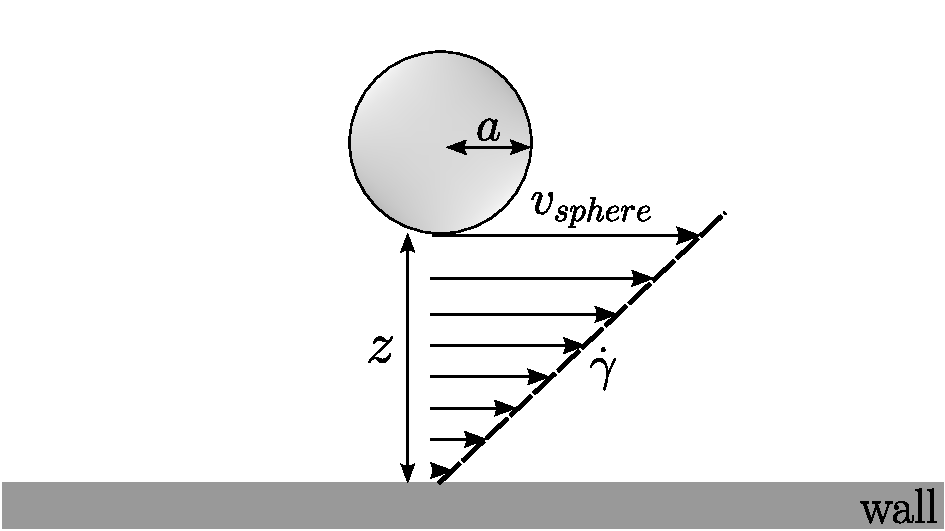
\includegraphics{02_body/chapter3/images/draw_shear/shear.pdf}
	\caption{Schematic representation of a spherical colloid moving near a wall and the induced shear rate $\dot{\gamma}$.} 
	\label{fig.shear}
\end{figure}

A colloid diffusing near a wall thus experience a local drag force that depends on both it's distance to the wall $z$ and the movement direction. Thanks to the linearity of the Stokes equation, one can seperate this local drag force for motion parrallel and perpendicular to the wall. As the presence of the wall correct the drag force from a multiplicative coefficient, the confinement effect often expressed as an effective viscosity:

\begin{equation}
	\eta _\bot (z) = {\eta}{\lambda _ \bot (z)}  ~ \text{, and, } ~\eta _\parallel (z) =  {\eta}{\lambda _ \parallel (z)}~,
\end{equation}

where $\lambda _\bot$ and $\lambda _\parallel$ are respectively perpendicular and parallel correction factor to the drag force due to the presence of the wall. Due to this correction, the diffusion coefficients for parallel and perpendicular motion relative to the wall writes:

\begin{equation}
	D_\bot (z) =  \frac{D_0}{\lambda _\bot (z)}  ~, \text{ and, } D_\parallel (z) = \frac{D_0}{ \lambda_\parallel (z)} ~.
\end{equation}
 
For a no-slip boundary conditions imposed at the wall and the surface of the colloid, Brenner \cite{brenner_slow_1961} obtained for perpendicular motion:


\begin{equation}
	\lambda_ \bot (z) = \frac{4}{3}  \mathrm{sinh}\beta \sum _{n=1} ^{\infty} \frac{n(n+1)}{(2n-1)(2n+3)}
	\left[
	\frac
	{
		2\mathrm{sinh}(2n + 1)\beta + (2n +1)\mathrm{sinh}2\beta
	}
	{
		4\mathrm{sinh}^2(n + 1 /2)\beta  - (2n+1)^2 \mathrm{sinh}^2 \beta
	}
	-1
	\right] ~,
	\label{Eq:etaz}
\end{equation}

where $\beta = \cosh ^{-1} ((z+a)/a)$. The solution for the diffusion parallel to the wall, Faxén found \cite{faxen_fredholm_1924}:

\begin{equation}
	\lambda_\parallel(z) = 
	\left[
	1 - \frac{9}{16} \xi + \frac{1}{8}\xi^3 - \frac{45}{256}\xi^4 - \frac{1}{16}\xi^5
	\right]^{-1}~,
	\label{Eq:etax}
\end{equation}

where $\xi  = a / (z+a)$. Eqs.\ref{Eq:etaz} and \ref{Eq:etax} are precise for all $z$. However, the solution for the perpendicular motion can be quite complex to compute as it is an infinite series, to be computed numerically it requires a software that enable arbitrary-precision floating-point arithmetic\footnote{Arbitrary-precision floating-point arithmetic enables to evaluate mathematical expression with any precision, in other words, any number of digits.} --- such as Mathematica or the \mintinline{python}{mpmath} Python's module for example. $D_\bot$ can be evaluated using the following Python snippet, where \mintinline{python}|nsum| function is used to compute the infinite sum:  


\begin{minted}
	[
	frame=lines,
	framesep=2mm,
	baselinestretch=1.2,
	fontsize=\footnotesize,
	linenos
	]
	{python}
from mpmath import nsum	

def Dz(eta, z, a):
  a = (z + a) / a
  beta = float(acosh(a))
  summ = nsum(
    lambda n: (n * (n + 1) / ((2 * n - 1) * (2 * n + 3)))
    * (
      (
        (2 * sinh((2 * n + 1) * xi) + (2 * n + 1) * sinh(2 * beta))
        / (
            4 * (sinh((n + 1 / 2) * beta) ** 2)
            - ((2 * n + 1) ** 2) * (sinh(beta) ** 2)
        )
      )
      - 1
    ),
    [0, inf],
    )
  summ = float(summ)
  return kT / (6 * pi * eta * 4 / 3 * float(sinh(beta)) * summ * a)
\end{minted}

To simplify the computation of $\lambda_\bot$, Goldman \textit{et al.} \cite{goldman_slow_1967} showed that Eq.\ref{Eq:etaz} can be Padé approximated, giving:

\begin{equation}
	\lambda_\bot =  \frac{6z^2 + 9az + 2a^2}{6z^2 + 2az}~.
	\label{Eq:etaz_pade}
\end{equation}

In the near-wall regime, such that $z \ll a$, it is also possible to further approximate $\lambda_\bot$ to:

\begin{equation}
	\lambda_\bot = \frac{a}{z} ~.
	\label{Eq:etaz_small}
\end{equation}


\begin{figure}[H]
	\centering
	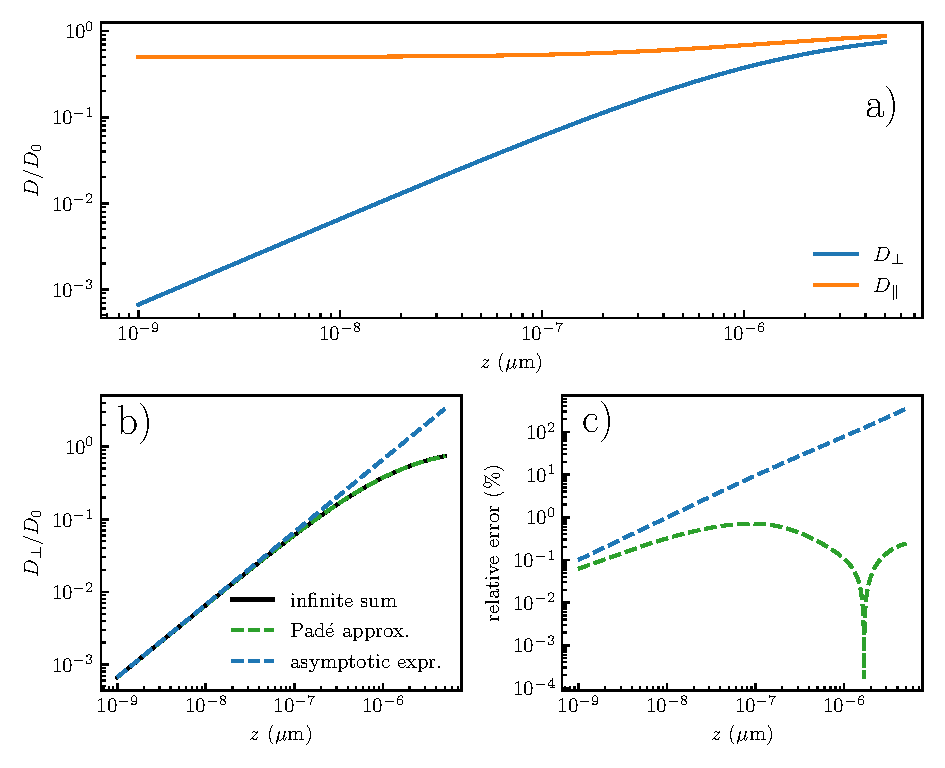
\includegraphics{02_body/chapter3/images/theory_lambda/hindered_diffusion.pdf}
	\caption{a)  Parallel and perpendicular hindered relative diffusion coefficient for a colloidal particle of radius $a = 1.5 ~ \mathrm{\mu m}$. b) Perpendicular hindered relative diffusion coefficient for a colloid particle of radius $a = 1.5 \mathrm{mu m}$. In black the exact solution given by the infinite sum Eq.\ref{Eq:etaz}. In green the Padé approximation, Eq.\ref{Eq:etaz_pade} and in blue the near wall regime Eq.\ref{Eq:etaz_small}. c) Relative error of the perpendicular hindered coefficient.}
	\label{fig.etaz}
\end{figure}


The Padé approximation and the near-wall approximation for the hindered diffusion are plotted on Fig.\ref{fig.etaz}-b). The Padé approximation fits really well with the exact solution given by the infinite sum Eq.\ref{Eq:etaz}, the near-wall approximation fits well when $z < a / 10$. To check how precise the approximation are, it is possible to plot the relative error as in the Fig.\ref{fig.etaz}-c). The Padé approximation shows a precision up to 1\%, thus, in the following of this work, when we refer to any evaluation of the hindered perpendicular diffusion, the Padé approximation will be used. 


\subsubsection{Langevin equation for the confined Brownian motion}

Now that the external forces acting on the particle and hindered diffusion coefficient is known, we rewrite the overdamped Langevin Eq.\ref{Eq.overdamped_SDE} equation as:

\begin{equation}
	V_t^i \textnormal{d}t  = -\frac{1}{\gamma(z)}\frac{\partial U(z)}{\partial x_i}  \textnormal{d}t + \sqrt{2D_i (z)}  \textnormal{d}B_t ~.
	\label{Eq:langevin_z}
\end{equation}

where $\gamma(z) = 6 \pi \eta_i(z) a$ and $i$ denotes three spatial directions, $x,~ y$ and $z$\footnote{Where the previously determined $\eta_\parallel$ and $D_\parallel$ correspond to the $x$ and $y$ axis and $\eta_\bot$ and $D_\bot$ correspond to the $z$ axis.}, and,  $ \textnormal{d}B_t$ still is a Gaussian distribution satisfying $\langle \textnormal{d}B_t \rangle = 0$ and $\langle \textnormal{d}B_t ^2 \rangle = \textnormal{d}t$. As we have discussed previously, the potential $U$ only varies along the $z$ axis, thus, the external forces only acts on the particle on the $z$ axis while the particle diffuses freely along the $x$ and $y$ axis. 

\subsubsection{Spurious drift}

It is interesting to observe that due to the hindered diffusion the magnitude of the Langevin force, $\sqrt{2D_i(z)}$, is not anymore a constant, but varies with the height of the particle. This effect is called multiplicative noise and will have some interesting effects on the dynamics properties of the Brownian motion. To show the effects of the multiplicative noise, one can integrate over a time $\tau$ the Eq.\ref{Eq:langevin_z}, in the absence of the external force one has:

\begin{equation}
	\Delta x_i = \int_{t_0} ^{t_0 + \tau} \sqrt{2D_i(z)}\textnormal{d}B_t
	\label{int}
\end{equation}

where $\Delta x_i$ is a space increment. However, the noise term is not well-defined and the time at which the magnitude of the force $\sqrt{2D_i(z)}$ in the integration Eq.\ref{int} needs to be specified. It is thus necessary to determine where the Diffusion coefficient $D(z)$ in Eq.\ref{int} is evaluated in the time interval $[t_0, t_0 + \tau]$. In general, $D(z)$ is represented by $D(z + \alpha \Delta z)$, or in the same way $D(z(t_0 + \alpha \tau))$, with $\alpha \in [0,1]$. The value of $\alpha$ determines at which time in the interval   $[t_0, t_0 + \tau]$ the local diffusion is evaluated, hence, the magnitude of the random force. The physics will thus change on how the noise is calculated, however, the requirement is that the long-time thermal equilibrium must be consistent with the Boltzmann distribution and, hence, constrain the choice of $\alpha$. Taking into account $\alpha$, the langevin equation without external \ref{int} forces along the $z$ axis becomes:

\begin{equation}
	\Delta z  = \sqrt{2D_\parallel (z + \alpha \Delta z)} d B_t ~.
	\label{int2}
\end{equation}

By Taylor expendig $D_ \parallel$ to the first order one has:

\begin{equation}
	D_\parallel (z + \alpha \Delta z) \simeq D_\parallel (z)  + \alpha \frac{\textnormal{d} D_\parallel(z)}{\textnormal{d}z} \Delta z ~.
\end{equation}

Substituting the later in Eq.\ref{int2} leads to:

\begin{equation}
	\begin{aligned}
		\Delta z &\simeq \sqrt{2D_\parallel (z)  + \alpha \frac{\textnormal{d} D_\parallel(z)}{\textnormal{d}z} \Delta z} d B_t  \\
		& = \sqrt{2D_\parallel (z)} \left[1 + \alpha \frac{\textnormal{d} D_\parallel(z)}{\textnormal{d}z} \frac{\Delta z }{D_\parallel(z)}\right] ^{-1/2} \textnormal{d} B_t  ~.
	\end{aligned}
	\label{int3}
\end{equation}

Additionally, since the last term satisfies:

\begin{equation}
	\alpha \frac{\textnormal{d} D_\parallel(z)}{\textnormal{d}z} \frac{\Delta z }{D_\parallel(z)} \ll 1 ~,
\end{equation}

one can thus Taylor expend at the first order the last term of Eq.\ref{int3} as:

\begin{equation}
	\left[1 + \alpha \frac{\textnormal{d} D_\parallel(z)}{\textnormal{d}z} \frac{\Delta z }{D_\parallel(z)}\right] ^{-1/2} \simeq 1 + \frac{\alpha }{2}\frac{\textnormal{d} D_\parallel(z)}{\textnormal{d}z} \frac{\Delta z }{D_\parallel(z)} ~.
\end{equation}

By finally substituting the first-order expansion of $\Delta z \simeq \sqrt{2D(z)} \textnormal{d}B_t$, we obtain:

\begin{equation}
	\begin{aligned}
		\Delta z & \simeq \sqrt{2D_\parallel (z)} \left[1 + \frac{\alpha }{2} \frac{\textnormal{d} D_\parallel(z)}{\textnormal{d}z} \frac{\Delta z }{D_\parallel(z)}\right]  \textnormal{d} B_t \\
		& \simeq \sqrt{2D_\parallel (z)} \left[1 + \frac{\alpha }{2} \frac{\textnormal{d} D_\parallel(z)}{\textnormal{d}z} \frac{\sqrt{2D(z)} \textnormal{d}B_t }{D_\parallel(z)}\right]  \textnormal{d} B_t \\
		& =  \sqrt{2D_\parallel (z)} \textnormal{d}B_t + \alpha  \frac{\textnormal{d} D_\parallel(z)}{\textnormal{d}z} \textnormal{d} B_t ^2
	\end{aligned}
\end{equation}



Since for short time $\textnormal{d}B_t \rightarrow 0$ it is possible to replace $\textnormal{d}B_t ^2$ by its average value  $\langle \textnormal{d}B_t ^2 \rangle _t = \tau$, the latter thus become \cite{ikeda_stochastic_2014}: 

\begin{equation}
	\begin{aligned}
	\Delta z &=   \alpha  \frac{\textnormal{d} D_\parallel(z)}{\textnormal{d}z}  \tau - \frac{1}{\gamma(z)}\frac{\partial U(z)}{\partial z}  \tau + \sqrt{2D_\parallel (z)} \textnormal{d}B_t \\
	&=  \left( - \frac{1}{\gamma(z)}\frac{\partial U(z)}{\partial z} +  \alpha  \frac{\textnormal{d} D_\parallel(z)}{\textnormal{d}z} \right) \tau + \sqrt{2D_\parallel (z)} \textnormal{d}B_t \\
	&= \bar{v}_\textnormal{d}\tau  + \sqrt{2D_\parallel (z)} \textnormal{d}B_t ~,
	\end{aligned}
\end{equation}

where:

\begin{equation}
	\bar{v}_\textnormal{d} = - \frac{1}{\gamma(z)}\frac{\partial U(z)}{\partial z} +  \alpha  \frac{\textnormal{d} D_\parallel(z)}{\textnormal{d}z}  = v_\textnormal{d} + v_\textnormal{noise}~,
	\label{Eq.total_drifts}
\end{equation}

are the total drifts acting on the particle. The first term $v_\textnormal{d}$ is the drift  due to ``real" deterministic forces due to the electrostatic double-layer and gravity interactions, while the second term $ v_\textnormal{noise}$ represents a noise induced drift. This spurious drift does disappear when the coefficient diffusion is homogeneous as for the $x$ and $y$ axis as the coefficient diffusion only depends on the colloid's height. Theoretically, $\alpha$ can take any value between 0 and 1. However, $\alpha$ generally takes 3 different values \cite{volpe_effective_2016}:  $\alpha = 0$, the Itô integral, coresponding to the use of the initial value of $D(z)$; $\alpha = 1/2$, the Stratonovich integral, corresponding to the mid-point value; and $\alpha = 1$ the anti-Itô or isothermal integral, corresponding to the use of the final value. 

In particular, the Itô integral $\alpha = 0$ is commonly used in economics and biology as integrals are approximated by a sum, the first point of the integral is chosen.  The Stratonovich integral $\alpha = 1/2$ arises in Physical systems where noise correlation time $\tau _\mathrm{c} > 0$, and, where the velocities are often computed at mid-points using three measurements. Finally, the isothermal integral $\alpha = 1$ is used in physical systems at equilibrium with a heat bath \cite{volpe_influence_2010} such as our case with Brownian motion. Using the Padé approximation Eq.\ref{Eq:etaz_pade}, the spurious drift $v_\textnormal{noise}$ writes:

\begin{equation}
	v_\textnormal{noise} (z)= 2 \alpha D_0 a\frac{2a^2 + 12 az + 21 z^2}{(2 a^2 + 9az + z^2) ^2} ~,
	\label{Eq.spurious_drift}
\end{equation}

and the deterministic part of the drift writes:

\begin{equation}
	v_\textnormal{d} =- \frac{k_\mathrm{B}T}{\gamma(z)} \left[- \frac{1}{\ell_\mathrm{D}} B \exp \left(- \frac{z}{\ell_\mathrm{D}}\right) + \frac{1}{\ell_\mathrm{B}}\right] ~.
\end{equation}

A typical example of drift velocity for a colloidal particle of radius $a = 1.5 ~\mathrm{\mu m}$ in water, confined in interaction potential with a Debye length $\ell_\mathrm{D} = 50 ~ \mathrm{nm}$, $B = 4 ~k_\mathrm{B}T$ and a Boltzmann length $\ell_\mathrm{B} = 500 ~ \mathrm{nm}$, is plotted in Fig.\ref{fig.spurious}. As one can observe, the spurious drift is not negligible, and, even the presence of this additional drift doubles the total drift $\bar{v}_\mathrm{d}$ near the surface.
\begin{figure}[ht]
	\centering
	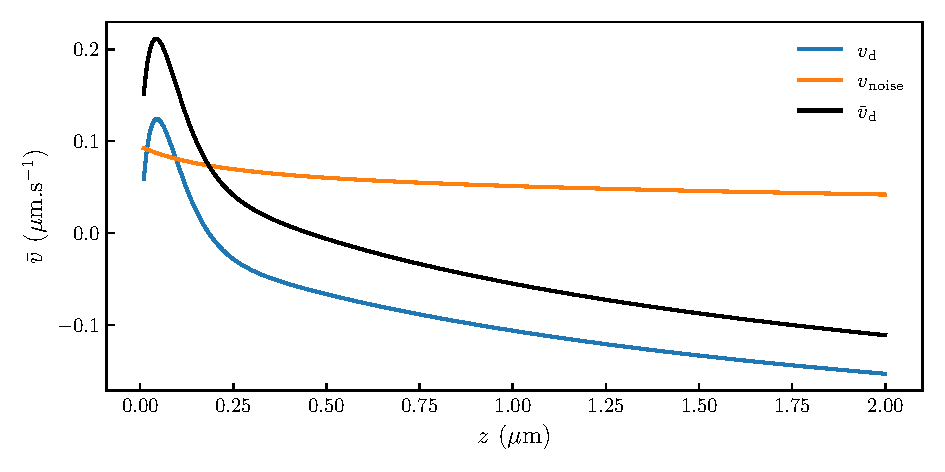
\includegraphics{02_body/chapter3/images/spurious_drift/spurious.pdf}
	\caption{Typical drift velocity for a confined colloidal particle of radius $a = 1.5 ~\mathrm{\mu m}$ in water. The physical properties of the interaction are $\ell_\mathrm{D} = 50 ~ \mathrm{nm}$, $B = 4 ~k_\mathrm{B}T$ and $\ell_\mathrm{B} = 500 ~ \mathrm{nm}$.} 
	\label{fig.spurious}
\end{figure}

\subsubsection{Fokker-Plank equation}

The Fokker-Plank equation is an alternative way to describe Brownian motion. Instead of explicitly calculating a Brownian trajectory by solving the Langevin equation, Fokker-Plank equation describes the particle distribution function $P(x, x_0; t)$ where $x$ denotes the particle position and $x_0$ its initial position. To derive the Fokker-Plank plank equation, let us start by taking generic Langevin equation:

\begin{equation}
	\textnormal{d}X_t = u(X_t) \textnormal{d}t + a(X_t)\textnormal{d}B_t ~,
	\label{SDE2}
\end{equation}

where $X_t$ is the particle position,  $u$ is the drift due to external forces and $a$ the magnitude of the random force. Let consider the average value of an arbitrary function $f(X_t)$ for a stochastic process obeying Eq.\ref{SDE2}, that started at position $x_0$ at time $t=0$, by definition \cite{le_bellac_equilibrium_2004}:

\begin{equation}
	\langle f(X_t) \rangle = \int \textnormal{d}x ~ p(x, x_0 ; t) f(x) ~,
	\label{fokker1}
\end{equation}

with the initial conditions that can be written as:

\begin{equation}
	p(x, x_0; 0) = \delta (x - x_0) ~.
\end{equation}

We now take the time derivative of Eq.\ref{fokker1}, we start by expending $ f$ at the $\textnormal{d}t$ as:

\begin{equation}
	\begin{aligned}
	\left\langle \frac{\textnormal{d}f(X_t)}{\textnormal{d}t} \right\rangle  &= \frac{\textnormal{d}}{\textnormal{dt}}\left\langle   \frac{\partial f(X_t)}{\partial x} u(X_t) \textnormal{d}t + \frac{1}{2} \frac{\partial^2 f(X_t)}{\partial x^2} a^2 (X_t) \textnormal{d}B_t^2   \right\rangle \\
	& =  \frac{\textnormal{d}}{\textnormal{dt}} \left( \frac{\partial f(X_t)}{\partial x} u(X_t) \textnormal{d}t + \frac{1}{2} \frac{\partial^2 f(X_t)}{\partial x^2} a^2 (X_t) \textnormal{d}t \right) \\
	& = \frac{\partial f(X_t)}{\partial x} u(X_t) + \frac{1}{2} \frac{\partial^2 f(X_t)}{\partial x^2} a^2 (X_t) ~.
	\end{aligned}
	\label{fokker2}
\end{equation}

By combining Eqs.\ref{fokker1} and \ref{fokker2}, we get:

\begin{equation}
	\begin{aligned}
	\left\langle \frac{\textnormal{d}f(X_t)}{\textnormal{d}t} \right\rangle &= \int \textnormal{d} x ~\frac{\partial p(x, x_0 ; t) }{\partial t} f(x) \\
	& =  \frac{\partial f(X_t)}{\partial x} u(X_t) + \frac{1}{2} \frac{\partial^2 f(X_t)}{\partial x^2} a^2 (X_t) \\
	& = \int \textnormal{d}x ~ p(x, x_0 ; t) G f(x) ~,
	\end{aligned}
\end{equation}

where G in an operator called the generator and is define by its action on a function $f$ by:

\begin{equation}
	Gf = \frac{1}{2} a^2 (x) \frac{\partial ^2 f(x)}{\partial x^2} + u(x) \frac{\partial f(x)}{\partial x} ~.
\end{equation}

Using the definition of the adjoint of $G$, denoted by $G ^\dagger$, one has:


\begin{equation}
	\begin{aligned}
	\int \textnormal{d} x ~\frac{\partial p(x, x_0 ; t) }{\partial t} f(x) &= \int \textnormal{d}x ~ p(x, x_0 ; t) G f(x) \\
	&= \int \textnormal{d}x ~  G ^\dagger p(x, x_0 ; t) f(x) ~.
	\end{aligned}
\end{equation}

From the latter, we thus have:

\begin{equation}
	\frac{\partial p(x, x_0 ; t)}{\partial t} = G^\dagger p(x, x_0 ; t) ~.
	\label{fokker3}
\end{equation}

Which leads to the Forward-Fokker-Planck equation:

\begin{equation}
	\frac{\partial p(x, x_0 ; t)}{\partial t }= \frac{\partial ^2}{\partial x^2} \left[\frac{a^2 (x)}{2}p(x, x_0 ; t)\right] - \frac{\partial}{\partial x} \left[u(x) p(x, x_0 ; t)\right]
	\label{Eq.Forward_Fokker_plank}
\end{equation}

The latter is called Forward because the partial differential equation is in terms of the variable $x$, the position of the particle at which the stochastic process ends up, at time $t$. For a confined Brownian motion near a wall, using the previously determined drifts $\bar{v}_\textnormal{d}$ Eq.\ref{Eq.total_drifts}, the Fokker-Plank equation for the movement along the $z$ axis, perpendicular to the wall writes:

\begin{equation}
	\frac{\partial p(z, z_0 ; t)}{\partial t} = \frac{\partial ^2}{\partial z ^2} \left[ D(z)  p(z, z_0 ; t) \right]   -  \frac{\partial }{\partial z} \left[\bar{v}_\textnormal{d} p(z, z_0 ; t)\right] ~.
\end{equation}

As an example, the stationary solution of the latter, $\partial p / \partial t = 0$, is given by the Gibbs-Boltzmann ditribution $P_\textnormal{eq}(z) $ (Eq.\ref{Eq.Peq}). The solution for the Eq.\ref{fokker3} with the particle starting at position $z_0$, at time $t_0 = 0$ writes:

\begin{equation}
	\begin{aligned}
	P(z, z_0; t) &= \exp (G^\dagger t) p(z, z_0, 0) \\
	& = \exp \left( \frac{\partial ^2}{\partial z ^2}  D(z)  t   -  \frac{\partial }{\partial z} \bar{v}_\textnormal{d} t\right) \delta (z - z_0)
	\end{aligned}
\end{equation} 

\subsubsection{Numerical simulation of confined Brownian motion}

We had previously determined with that the simulation of a bulk Brownian motion, without external forces can by the simple formula (Eq.\ref{Eq.shortnumlangevin}): 

\begin{equation}
	x_i = x_{i-1} + \sqrt{2D}w_i~.
\end{equation}

However, with the confined Brownian motion one needs to take into account the hindered diffusion, external forces due to gravity and double-layer interactions and the noise-induced drift. Putting all that together, leads to a new equation for $x_i$ which writes for the movement parrallel to wall:

\begin{equation}
	x_i = x_{i-1} +  \sqrt{2D_\parallel}w_i ~,
\end{equation}

where $i$ represents $x$ and $y$ axis. For the particle movement perpendicularly to the wall ($z$ axis), one needs to add the total drift $\bar{v}_\textnormal{d}$ Eq.\ref{Eq.total_drifts}, such that:

\begin{equation}
	z_i = z_{i-1} + \bar{v}_\mathrm{d}(z_{i-1}) \tau + \sqrt{2D_\bot}w_i ~,
\end{equation}

where $\tau$ is the simulation time step and $w_i$ being a Gaussian distribution of mean value $\langle w_i \rangle = 0$ and variance $\langle w_i ^2\rangle = \tau$. Unlike the bulk Brownian motion where the time step $\tau$ can be chosen for the desired precision as shown previously on Fig.\ref{fig:MSEwi}; for an accurate simulation, the time-step should here be short enough for the drifts $\bar{v}_\textnormal{d}$ and local diffusion coefficient to be relatively constant in the time periods $t_{i+1} - t_i = \tau$ and in the displacement range $\Delta z = z_{i+1} - z_i$, such that:

\begin{equation}
	\bar{v}_\mathrm{d} (z \in [z_i, z_{i+1}]) \simeq \bar{v}_\mathrm{d} (z_i) ~,
	\label{driftc}
\end{equation}

and,

\begin{equation}
	D_{\bot, \parallel}(z \in [z_i, z_{i+1}]) \simeq D_{\bot, \parallel}(z_i) ~.
\end{equation}

Since that the diffusion coefficient vary less for the movement parallel one can only consider the perpendicular motion to determine the simulation time step. Also, as it can be seen on the Fig.XX where the drift $v_\textnormal{d}$ and diffusivity gradient are plotted, the diffusion gradient are negligible compared to the drift gradient, we thus focus on the drifts condition Eq.\ref{driftc}. Moreover, the drifts vary more when the colloid is near the surface where one can approximate the diffusion coefficient $D_\bot$ by the approximation Eq.\ref{Eq:etaz_small} such that:

\begin{equation}
	D_\bot ^{z\ll a} (z) = D_ 0 \frac{z}{a} ~.
\end{equation}

As near the surface, the gravitational interaction can be neglected as it is smaller that the electrostatic interactions has it has been shown on the potential plot Fig.\ref{Fig:potential}. In that case, by taking $\alpha = 1$, the total drifts Eq.\ref{Eq.total_drifts} near the surface simplifies to:

\begin{equation}
	\begin{aligned}
		\bar{v}_\textnormal{d} &=  \frac{k_\mathrm{B}T}{\gamma_0} \frac{z}{a} \left[\frac{B}{\ell_\mathrm{D}} \exp \left(-\frac{z}{\ell_\mathrm{D}}\right)\right] + \frac{\partial}{\partial z} D_0 \frac{z}{a} \\
		&= D_0 \frac{z}{a} \left[\frac{B}{\ell_\mathrm{D}} \exp \left(-\frac{z}{\ell_\mathrm{D}}\right)\right] + \frac{D_0}{a} \\
		&= \frac{D_0}{a} \left[ 1 + \frac{Bz}{\ell_\mathrm{D}} \exp \left(-\frac{z}{\ell_\mathrm{D}}\right)\right]
	\end{aligned}
\end{equation}

By expending the exponential term to the order $z/\ell_\mathrm{D}$ order, we get:

\begin{equation}
	\begin{aligned}
		\bar{v}_\textnormal{d} &= \frac{D_0}{a} \left[ 1 + \frac{Bz}{\ell_\mathrm{D}} \exp \left(-\frac{z}{\ell_\mathrm{D}}\right)\right]
		 =  \frac{D_0}{a} \left[ 1 + \frac{Bz}{\ell_\mathrm{D}}  \left(1 -\frac{z}{\ell_\mathrm{D}}\right)\right] \\
		& = \frac{D_0}{a} \left( 1 + \frac{B z}{\ell_\mathrm{D}}\right)
	\end{aligned}
	\label{drifts_short}
\end{equation}

To satisfy Eq.\ref{driftc}, we need to have small relative change of drifts in an interval $[z, z+\Delta z]$ which can be written as:

\begin{equation}
	\frac{\bar{v}_\mathrm{d} (z + \Delta z) - \bar{v}_\mathrm{d} (z)}{\bar{v}_\mathrm{d} (z)} \ll 1
	\label{condition_drift}
\end{equation}

Combining Eqs.\ref{drifts_short} and \ref{condition_drift}, we get:

\begin{equation}
	\Delta z \ll \frac{\ell_\mathrm{D}}{B} + z ~.
	\label{inegality}
\end{equation}


Using the \gls{MSD}, it is possible to link the latter to the simulation time step $\tau$ by using the average value of $\Delta z ^2 $, such that:

\begin{equation}
	\langle \Delta z ^2 \rangle (z) = 2 D_\bot (z) \tau = 2D_0 \frac{z}{a}\tau 
	\label{msdshort}
\end{equation}

Combining Eqs.\ref{inegality} and \ref{msdshort} thus leads to:

\begin{equation}
	\tau = \frac{a\langle \Delta z ^2 \rangle }{2 D_0 z} < \frac{a}{2 D_0 } \frac{(\frac{\ell_\mathrm{D}}{B} + z) ^2}{z} = \tau_\mathrm{max} (z)~,
	\label{taumax}
\end{equation}

where $ \tau_\mathrm{max}$ is thus the maximal time step that satifies Eq.\ref{inegality}. At this point, there is two different way to do the simulation: the first one is to do an adaptive time step where $\tau_\mathrm{max}$ for each step of the simulation ; the second one is to find the smallest $\tau_\mathrm{max}(z)$ and use for all the simulation a time step $\tau$ statisfying $\tau < \mathrm{min}(\tau_\mathrm{max}) $. The latter can be evaluated by finding the height $z_\mathrm{min}$, at which the derivative of $ \tau_\mathrm{max}$ nullifies, such that:

\begin{equation}
	\left. \frac{\partial \tau_\mathrm{max}}{\partial z} \right| _{z_\mathrm{min} }= 0 ~.
\end{equation} 

Soliving the latter gives:

\begin{equation}
	z_\mathrm{min} = \frac{\ell_\mathrm{D}}{B} ~.
\end{equation}


which finally gives a maximal simulation time step, $\mathrm{min}(\tau_\mathrm{max})$:

\begin{equation}
	\mathrm{min}(\tau_\mathrm{max}) =  \frac{2 a}{D_0} \frac{\ell_\mathrm{D}}{B} ~,
\end{equation}

this time should be the maximal time step $\tau$ used for a confined Brownian simulation near a wall to ensure an accurate simulation of the near-wall effects. In the Fig.\ref{fig.taumax}-b) some typical $\tau_{\mathrm{max}}$ are plotted for a colloid of radius $a=1.5 ~\mathrm{\mu m}$, $B = 4$ and $\ell _\mathrm{D}$ varying between $20$ and $100$ nm. We can observe that for this range of values that well represents the experiments that I have done during my thesis, taking a simulation time step $\tau < 0.01 ~ \mathrm{s}$ can be used for all set of parameters.

\newpage

\begin{figure}[ht]
	\centering
	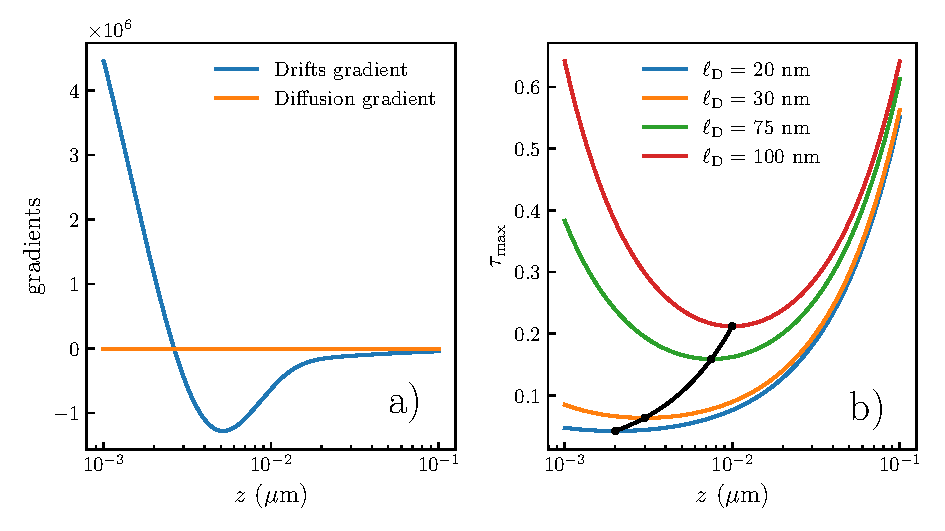
\includegraphics{02_body/chapter3/images/simulation_confined_Brownian_motion/maximal_tau.pdf}
	\caption{a) Drift and diffusive gradients for a confined colloidal particle of radius $a = 1.5 ~\mathrm{\mu m}$ in water. The physical properties of the interaction are $\ell_\mathrm{D} = 50 ~ \mathrm{nm}$, $B = 4 ~k_\mathrm{B}T$ and $\ell_\mathrm{B} = 500 ~ \mathrm{nm}$. b) $\tau_\mathrm{max}$ for a particle of radius $a = 1.5 ~\mathrm{\mu m}$ and $B = 4$ for different Debye length. The black line represent the minimum value $\tau_\mathrm{max}$ for $\ell_\mathrm{D}$ varying between 20 and 100 nm, this minimal time represent the maximal simulation time step that should be use for an accurate simulation.} 
	\label{fig.taumax}
\end{figure}

\begin{figure}[H]
	\centering
	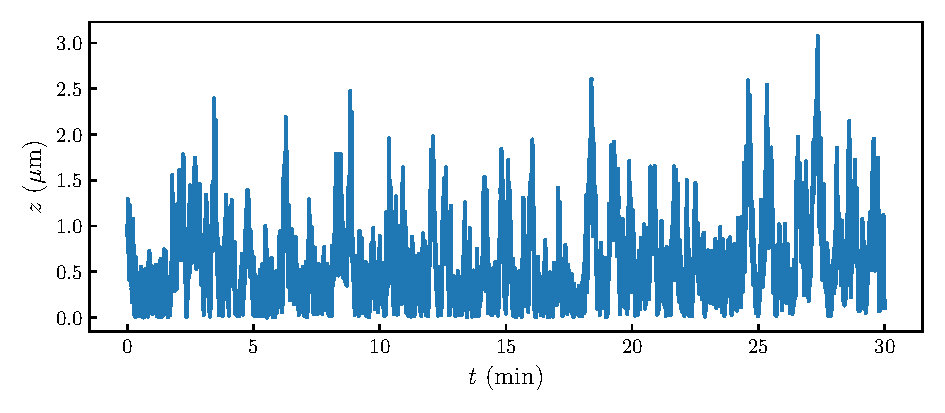
\includegraphics{02_body/chapter3/images/simulation_confined_Brownian_motion/z_traj_sim.pdf}
	\caption{Simulated confined Brownian motion height trajectory of a colloidal particle of radius $a= 1.5  ~ \mathrm{\mu m}$ of density $\rho_\mathrm{p} = 1050  ~\mathrm{kg.m^{-3}}$, $\alpha = 1$ and  the potential is characterized by $\ell_\mathrm{D} = 50$ nm and $B=4$.} 
	\label{fig.z_traj_confined_simulated}
\end{figure}

We have developed the simulation of the Confined Brownian motion using Python, as part of the Master's internship of Élodie Millan, the interested reader will find more information on confined Brownian motion in more complex systems in her forthcoming thesis. A trajectory of a colloidal particle of radius $a= 1.5  ~ \mathrm{\mu m}$ of density $\rho_\mathrm{p} = 1050  ~\mathrm{kg.m^{-3}}$ and the potential characterized by $\ell_\mathrm{D} = 50$ nm and $B=4$,  is plotted in the Fig.\ref{fig.z_traj_confined_simulated} which do look like the experimental trajectory that was shown in Fig.\ref{Fig:exp_z_traj} as an introduction to the chapter. In this trajectory, the noise induced lift is taken in account by using the isothermal approach $\alpha =1 $. However, to check if it is the correct way to take into account the spurious drift, the constraint we have is that the long time statistics should satisfy the Gibbs-Boltzmann equation Eq.\ref{Eq.Peq}. To compute an experimental probability density function from a set of points, one can use the following Python snippet.


\begin{minted}
	[
	frame=lines,
	framesep=2mm,
	baselinestretch=1.2,
	fontsize=\footnotesize,
	linenos
	]
	{python}
def pdf(data, bins=10, density=True):
	
  pdf, bins_edge = np.histogram(data, bins=bins, density=density)
  bins_center = (bins_edge[0:-1] + bins_edge[1:]) / 2

  return pdf, bins_center
\end{minted}

The Gibbs-Boltzmann distribution for $\alpha = 0 , 0.5 \text{ and } 1 $ is shown in Fig.\ref{fig.pdf_vs_alpha}. We see that the Isothermal integral of the noise gives the correct distribution, in the other two cases, we observe that the particle is more likely to be found nearer the surface, this is corrected by the additional spurious drift Eq.\ref{Eq.spurious_drift}.

\begin{figure}[hb]
	\centering
	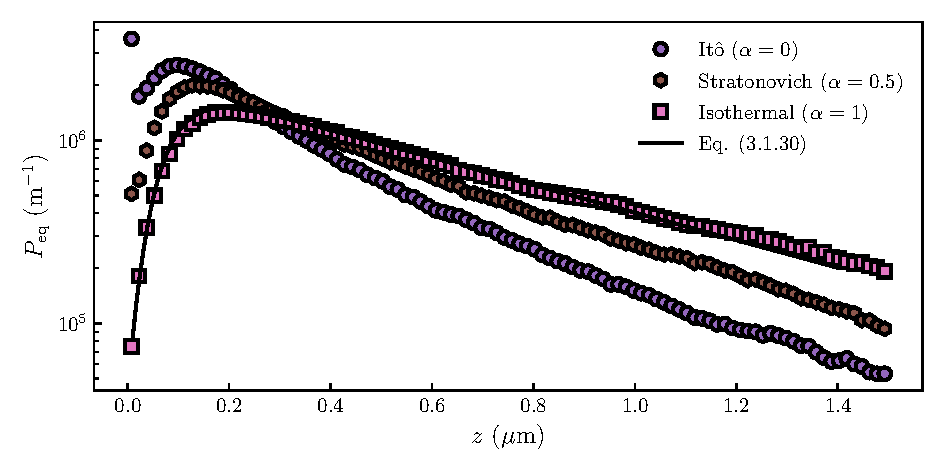
\includegraphics{02_body/chapter3/images/simulation_confined_Brownian_motion/Peq_vs_alpha.pdf}
	\caption{Probability Density Function of the height of the particle for different computation of the spurious drift, Itô $\alpha = 0$, Stratonovich $\alpha = 0.5$ and Isothermal $\alpha = 1$. The plain black line represents the expected Gibbs-Boltzmann distribution. The simulation parameters : $a = 1.5 ~ \mathrm{\mu m}$, $\rho_\mathrm{p} = 1050 ~\mathrm{kg.m^{-3}}$, $\ell_\mathrm{D} = 50$ nm, $B = 4$ and $\ell_\mathrm{B} = 577$ nm. }
	\label{fig.pdf_vs_alpha}
\end{figure}


\subsection{Experimental study}

\subsubsection{MSD}

\subsubsection{Non-gaussian dynamics - Displacement distribution}

\subsubsection{Local diffusion coefficient inference}

\subsubsection{Precise potential inference using multi-fitting technique}

\subsubsection{Measuring external forces using the local drifts}

\subsection{conclusion}
